\documentclass[12pt]{article}

\usepackage[spanish]{babel}
\usepackage{hyperref}
\usepackage{graphicx}
\usepackage{listings}
\usepackage{color}
\usepackage{multicol}
\usepackage{amssymb}

%% Título
\title{Matemáticas para las Ciencias Aplicadas I}

%% Fecha
\date{\today}

%% Autor
\author{Flores Morán Julieta Melina \\ Zarco Romero José Antonio}


%% Se marca el inicio del documento.
\begin{document}

%% Comando para crear el título.
\maketitle

%% Inicio de sección 1.
\section{Un cohete}
Un cohete es disparado verticalmente hacia arriba y el combustible que lo impulsa se quema durante 60 segundos. Se sabe que, a los $\Delta t$ s de haber iniciado su desplazamiento, la altura $h$ (en metros) a la que se encuentra el cohete es de 
\[h (t) = 40 t^2 ~ m\]

1. ¿A qué altura se halla el cohete cuando se le agota el combustible?
\[h (60) = 40 (60)^2 ~ m = 144000m\]

2. ¿Cuál es la rapidez promedio del cohete durante los primeros 60s de su vuelo?
\[
r = |v| = \frac{d}{t} = \frac{ 144000m}{60s} =  2400 m/s
\]

3. Haga una tabla con tres columnas: una para el tiempo $t$ (donde $t = 0, 10, 20, . . . , 60$), otra para la posición $h(t)$ y, una tercera para el incremento $\Delta h$ entre un valor de $t$ y el siguiente. Con base en ella, calcule la rapidez promedio del cohete para cada lapso de 10s desde $t = 0$ hasta $t = 60$.\\

%% Ejemplo de una tabla.
\begin{center}
\begin{tabular}{||c c c c||} 
 \hline
 $t$ & $h(t)$ &  $\Delta h$  & $v =\frac{\Delta h}{10}$ \\ [0.5ex] 
 \hline\hline
 0	& 0 & 0 & 0\\
10 & 	4000 &	4000 &	4000 \\
20	& 16000 &	12000	& 1200 \\
30 & 	36000	& 20000	& 2000 \\
40 & 	64000	& 28000 &	2800 \\
50	& 100000 & 	36000 &	3600 \\
60 & 	144000	& 44000	& 4400 \\ [1ex] 
\hline
\end{tabular}
\end{center}

4. Haga ahora otra tabla en la que muestre el cálculo de la rapidez promedio del cohete $\Delta t$ s antes y $t$ s después de $\Delta t $ = 3 s, para los siguientes valores de $t$:
\[
\frac{1}{10},\frac{1}{10 ^ 2} , \frac{1}{10 ^ 3}, \frac{1}{10 ^ 4}, \frac{1}{10 ^ 5}
\]

%% Ejemplo de una tabla.
\begin{center}
\resizebox{14cm}{!} {
\begin{tabular}{||c c c c c c c||} 
 \hline
  $\Delta t$ & $h(3- \Delta t)$ &  $h(3+ \Delta t)$ &  $\Delta h^-= h(3)-h(3- \Delta t)$ & $\Delta h^+ = h(3+ \Delta t) - h(3)$ & $v^- =\frac{\Delta h^-}{\Delta t}$  & $v^+ =\frac{\Delta h^+}{\Delta t}$  \\ [0.5ex] 
 \hline\hline
 $1$ 	& $h(2)=160$ & $h(4)=640$ & $360-160=200$ &  $640-360=280$ & $ \frac{200}{1}=200$ & $\frac{280}{1}=280$  \\ 
$ \frac{1}{10}$ & $h(2.9)=336.4$ & $h(3.1)=384.4$ & $336.4-160=23.6$ &  $640-384.4=24.4$ & $ \frac{23.6}{0.1}=236$ & $\frac{24.4}{0.1}=244$  \\ 
$ \frac{1}{10^2}$ & $h(2.99)=357.604$ & $h(3.01)=362.404$ & $360-357.604=2.396$ &  $362.404-360=2.404$ & $ \frac{2.396}{0.01}=239.6$ & $\frac{2.404}{0.01}=240.4$  \\ 
$ \frac{1}{10^3}$ & $h(2.999)=359.76004$ & $h(3.001)=360.24004$ & $360-359.76004=0.23996$ &  $360.24004-360=0.24004$ & $ \frac{0.23996}{0.0001}=239.96$ & $\frac{0.24004}{0.0001}=240.04$  \\ 
$ \frac{1}{10^4}$ & $h(2.9999)=359.9760004$ & $h(3.0001)=360.0240004$ & $360-359.9760004=0.0239996$ &  $360.0240004-360=0.0240004$ & $ \frac{0.0239996}{0.00001}=239.996$ & $\frac{0.0240004}{0.00001}=240.004$  \\
$ \frac{1}{10^5}$ 	& $h(2.99999)=359.97600004$ & $h(3.00001)=360.002400004$ & $360-359.97600004=0.002399996$ &  $360.0240004-360=0.002400004$ & $ \frac{0.002399996}{0.000001}=239.9996$ & $\frac{0.002400004}{0.000001}=240.0004$  \\ [1ex] 
\hline
\end{tabular}
}
\end{center}

5. Es razonable suponer que la rapidez instantánea del cohete exactamente a los $t = 3 s$, tome un valor intermedio entre la rapidez promedio $t$ s antes y $t$ s después de $t = 3$. Si esto es cierto, según sus cálculos, ¿cuánto vale esa rapidez instantánea?\\

La tabla muestra que tanto por la izquierda como por la derecha el valor se acerca a $240$, por lo que la velocidad instántanea en exactamente $3$ segundos debe ser $240 m/s$. Este valor es el valor obtenido al acercarnos lo más posible a $3$, por lo que podemos entender este como el límite cuando el tiempo tienda a $3$. 
\[
\lim_{t \to 3 }\frac{h(3)-h(t)}{3-t}=\lim_{t \to 3 }\frac{40(9)-40t^2}{3-t}=\lim_{t \to 3 }\frac{40(9-t^2)}{3-t}
\]

\[
\lim_{t \to 3 }\frac{40(3-t)(3+t)}{3-t}=\lim_{t \to 3 }40(3+t)=40(3+3)=40(6)=240
\]
%% Salto de página.
\clearpage

%% Sección 2.
\section{La pirámide del sol}
Según la Wikipedia, si se supone que la base de la pirámide del sol de Teotihuacan es cuadrada y que sus caras son lisas, su volumen es de
\[
1.184828 \times 10^6 m^3
\]
La versión en español de la misma informa que la altura de la pirámide es de $65$ m y el lado de su base mide $223 m$. A su vez, en la versión en inglés, se lee que la altura es de $71.17 m$ y el lado de la base mide $223.48 m$. ¿Cuáles son los datos congruentes con el valor del volumen propuesto arriba si se sabe que el volumen V de una pirámide viene dado por la fórmula
\\
(1)\\
\[
V =\frac{1}{3}Ah 
\]
donde <$A$ es el  área de la base y $h$, la altura? \\ \\
Versión en español:
\[
V =\frac{1}{3}(223m^2)(65m)=1.0774616666666 \times 10^6 m^3
\]
Versión en inglés:
\[
V =\frac{1}{3}(223.48m^2)(71.17m)=1.1848218003893 \times 10^6 m^3
\]
Entonces, las medidas de la versión en inglés se apegan más al volúmen.\\

Si bien la fórmula 1 se puede obtener mediante argumentos geométricos relativamente simples en los que no se aplica el método de \textit{rebanar, aproximar y pasar al límite} de Arquímedes, este ejercicio está orientado a experimentar numéricamente para encontrar una cota inferior y una cota superior del volumen V de la pirámide del sol; para ello, desarrolle los siguientes pasos:\\

1. Imagine que hace 49 cortes paralelos a la base, a intervalos regulares de longitud $ \Delta h = \frac{h}{50}$, donde $h$ es la altura de la pirámide, y suponga que el volumen $V_j$ de la j-ésima rebanada es aproximadamente igual
\begin{enumerate}
\item al volumen del prisma circunscrito a la pirámide de base cuadrada y altura $\Delta h$, para
j = 1, 2, . . . , 50;
\item al volumen del prisma inscrito en la pirámide de base cuadrada y altura $\Delta h$, para
j = 0, 1, . . . , 49;\\
\end{enumerate} 
2. Adapte el argumento que sugiere la siguiente figura (para el cálculo del volumen de un cono) al caso de la pirámide
\begin{figure}[h]
\centering
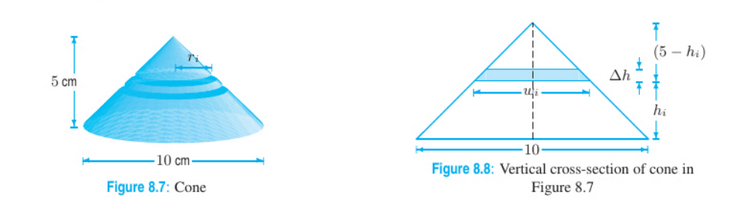
\includegraphics[ width=1\textwidth]{img/Partes.png}
\end{figure}

y aplíquelo para calcular los volúmenes $V_j$ de los prismas inscritos y circunscritos.\\

Para encontrar la fórmula que calcule los volúmenes $V_j$ de los prismas inscritos y circunscritos, debemos realizar lo siguiente:\\
Primero, necesitamos hallar la medida del lado de cada uno de ellos; de acuerdo con la semejanza de triángulos, sabemos que
\[
\frac{h_i}{h} = \frac{L_i/2}{L/2}
\]
Por lo tanto 
\[
L_i = \frac{L}{h} h_i 
\]
donde 
\[
h_i = h - (n_{partes} \cdot \Delta h)= h - (n_{partes} \cdot \frac{h}{50}) = h(1- \frac{n_{partes}}{50})
\]
Al sustituir $h_i$ en $L_i$, tenemos que
\[
L_i = \frac{L}{h} h_i = \frac{L}{h} \cdot h(1- \frac{n_{partes}}{50}) = L (1- \frac{n_{partes}}{50})
\]
donde $L=223.48m$
\[
\therefore L_i=223.48(1- \frac{n_{partes}}{50})m
\]
Al sustituir $L_i$ en la fórmula para el volumen de un prisma de base cuadrada $V=L^2 \cdot h$, obtenemos
\[
V=(223.48(1- \frac{n_{partes}}{50}))^2 \cdot h
\]
donde $h=\frac{71.17}{50}m=1.4234m$
\[
\therefore V_p=(223.48m(1- \frac{n_{partes}}{50}))^2 \cdot 1.4234m
\]
Aplicándola para calcular el volúmen de cada parte:

\begin{center}
\begin{tabular}{||c c c||} 
 \hline
 Parte & Lado $L_p (m)$ & Volumen $V_p (m^3)$\\ [0.5ex] 
 \hline\hline
$p0$ 	&	223.48	 &	71089.30802 \\
$p1$ 	&	219.0104	 &	68274.17143 \\
$p2$ 	&	214.5408	 &	65515.90627 \\
$p3$ 	&	210.0712	 &	62814.51257 \\
$p4$	 &	205.6016	 &	60169.99031  \\
$p5$ &	201.132	&	57582.3395 \\
$p6$	 &	196.6624 	&	55051.56013 \\
$p7$ &	192.1928	 &	52577.65221 \\
$p8$	 &	187.7232	 &	50160.61574 \\
$p9$	 &	183.2536	 &	47800.45071 \\
$p10$	 &	178.784	&	45497.15713 \\
$p11$	 &	174.3144 	&	43250.735 \\
$p12$	 &	169.8448	 &	41061.18431 \\
$p13$	 &	165.3752	 &	38928.50507 \\
$p14	$ &	160.9056	 &	36852.69728 \\
$p15 $	 &	156.436	&	34833.76093 \\
$p16$ 	 &	151.9664	 &	32871.69603 \\
$p17$	 &	147.4968	 &	30966.50257 \\
$p18$	 &	143.0272	 &	29118.18057 \\
$p19$	 &	138.5576	 &	27326.73 \\
$p20$	 &	134.088	 &	25592.15089 \\
$p21$	 &	129.6184	 &	23914.44322 \\
$p22$	 &	125.1488	 &	22293.607 \\
$p23$	 &	120.6792	 &	20729.64222 \\[1ex]
\hline
\end{tabular}


\begin{tabular}{||c c c||} 
 \hline
 Parte & Lado $L_p (m)$ & Volumen $V_p (m^3)$\\ [0.5ex] 
 \hline\hline
 $p24$	 &	116.2096	 &	19222.54889 \\
 $p25$ 	&	111.74	 &	17772.32701 \\  
$p26$ 	&	107.2704	 &	16378.97657 \\
$p27$	 &	102.8008	 &	15042.49758 \\
$p28$	 &	98.3312	 &	13762.89003 \\
$p29$	 &	93.8616	 &	12540.15394 \\
$p30$	 &	89.392	&	11374.28928 \\
$p31$	 &	84.9224	&	10265.29608  \\
$p32$	 &	80.4528	&	9213.17432 \\
$p33$	 &	75.9832	&	8217.924008  \\
$p34$	 &	71.5136	&	7279.545142 \\
$p35$	 &	67.044	&	6398.037722 \\
$p36$	&	62.5744	&	5573.401749 \\
$p37$	&	58.1048	&	4805.637222 \\
$p38$	&	53.6352	&	4094.744142 \\
$p39$	&	49.1656	&	3440.722508 \\
$p40$	&	44.696	&	2843.572321 \\
$p41$	&	40.2264	&	2303.29358 \\
$p42$	&	35.7568	&	1819.886285 \\
$p43$	&	31.2872	&	1393.350437 \\
$p44$	&	26.8176	&	1023.686036 \\
$p45$	&	22.348	&	710.8930802 \\
$p46$	&	17.8784	&	454.9715713 \\
$p47$	&	13.4088	&	255.9215089 \\
$p48$	&	8.9392	&	113.7428928 \\
$p49$	&	4.4696	&	28.43572321 \\
$p50$	&	0	&	0\\ [1ex] 
\hline
\end{tabular}

\end{center}

3. Sume los volúmenes que obtuvo en el inciso anterior y explique por qué el volumen de la pirámide del sol debe ser menor que la suma de los volúmenes de los prismas circunscritos y mayor que la suma de los volúmenes de los prismas inscritos.\\

Volúmenes de los primas circunscritos: 

\[
\sum_{i=0}^{49} V_{pc} = 1.22060341876 \times 10^6 m^3  
\]

Debe ser mayor que el volumen real, ya que todas las partes en que se dividió la pirámide tienen un excedente de la figura real.\\

Volúmenes de los primas inscritos:

\[
\sum_{i=1}^{50} V_{pi} = 1.14951411073 \times 10^6 m^3
\]

Debe ser menor al volumen real, ya que a las piezas en que se dividió les faltaba una parte para completar la figura de la pirámide. \\

\[
1.14951411073 \times 10^6 m^3 < V < 1.22060341876 \times 10^6 m^3 
\]

\[
\therefore \sum_{i=1}^{50} V_{pi} < V < \sum_{i=0}^{49} V_{pc}
\]

4. ¿Qué espera que suceda con estas cotas al hacer los mismos cálculos para un número de rebanadas más y más grande? 

Al rebanar la pirámide entre más piezas, lo esperado es que la suma de los volúmenes de los prismas, tanto circunscritos como inscritos, se aproximen al mismo valor. De esta manera, se obtendría el valor del volumen real de la pirámide cuando el número de las piezas tienda a infinito.
\clearpage

%sección 3
\section{Problema 22}
Un pequeño fabricante de electrodomésticos descubre que cuesta 9000 dólares producir 1000 tostadoras a la semana y 12000 dólares producir 1500 tostadoras a la semana.
\begin{enumerate}
\item Exprese el costo en función del número de tostadoras producidas, suponiendo que es lineal. Después, trace la gráfica.\\ 

Ya que suponemos que el costo $C$ es una función lineal del número de tostadoras $t$ de la forma $y = mx + b$, podemos escribir:

\[
	C=mt+b
\]

Utilizando los datos del problema, consideremos que conocemos los puntos (1000, 9000) y (1500, 12000). Por lo que la pendiente de la recta es

\[
	 m = \frac{\Delta {y}}{\Delta{x}} = \frac{12000-9000}{1500-1000} = \frac{3000}{500} = 6
\]

de modo que

\[
C=6t+b
\]

y su ecuación de la forma punto-pendiente $y-y_1=m(x-x_1)$, en el punto (1000, 9000) es 

\[
	C-9000=6(t-1000)
\]

o bien
\[
	C=6t+3000
\]

\[
\therefore f(t) = 6t + 3000
\]

Dicha ecuación da un posible modelo lineal, representado gráficamente como
\begin{figure}[h!]
\centering
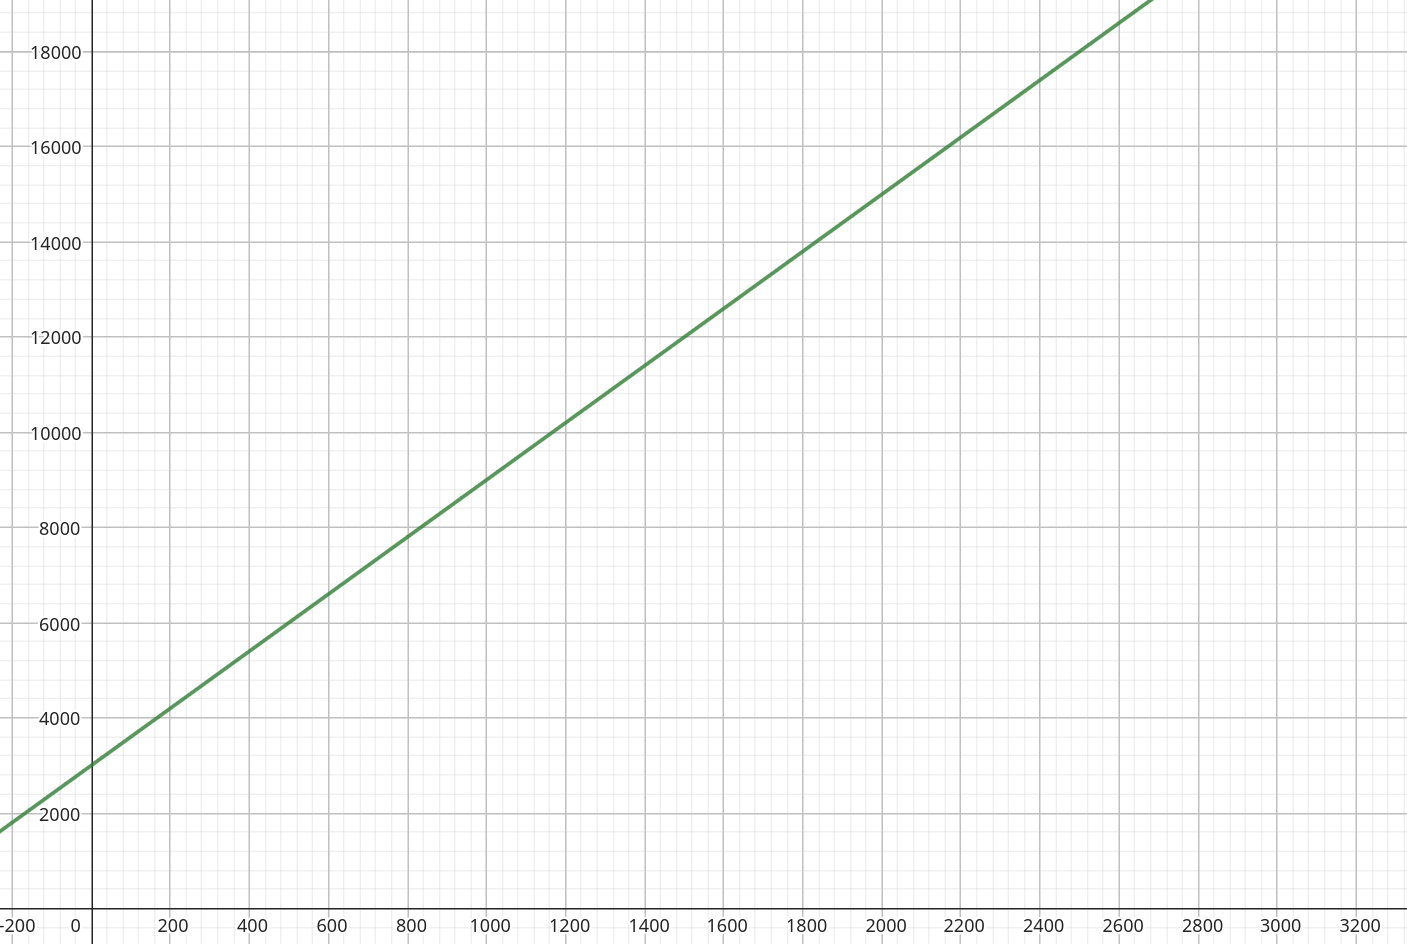
\includegraphics[width=10cm]{img/tostadoras.png}
\end{figure}

\item  ¿Cuál es la pendiente de la gráfica y qué representa?
\\ \\
La pendiente de la recta es $m=6$ y representa la razón de cambio, en este caso el aumento, del costo de producción en dólares respecto al número de tostadoras producidas.
\\  
\item  ¿Cuál es la intersección de la gráfica con el eje $y$ y qué representa?
\\
\[
f(0) = (6 \cdot 0) + 3000 = 3000
\]
La intersección con el eje $y$ es 3000 y representa el costo inicial de producción. No depende del número de tostadoras, es una constante sumada al costo independiente del número de tostadoras.
\\
\end{enumerate}

\clearpage
%sección 4
\section{Problema 27}
La población de ciertas especies en un ambiente limitado con una población inicial de 100 y capacidad para 1 000 es 
\[
P (t) = \frac{100 000}{100 + 900 e^{-t}} 
\]
donde t se mide en años.

\begin{enumerate}
\item Grafique esta función y estime cuánto tiempo le toma a la población llegar a 900.\\
\begin{figure}[h]
\centering
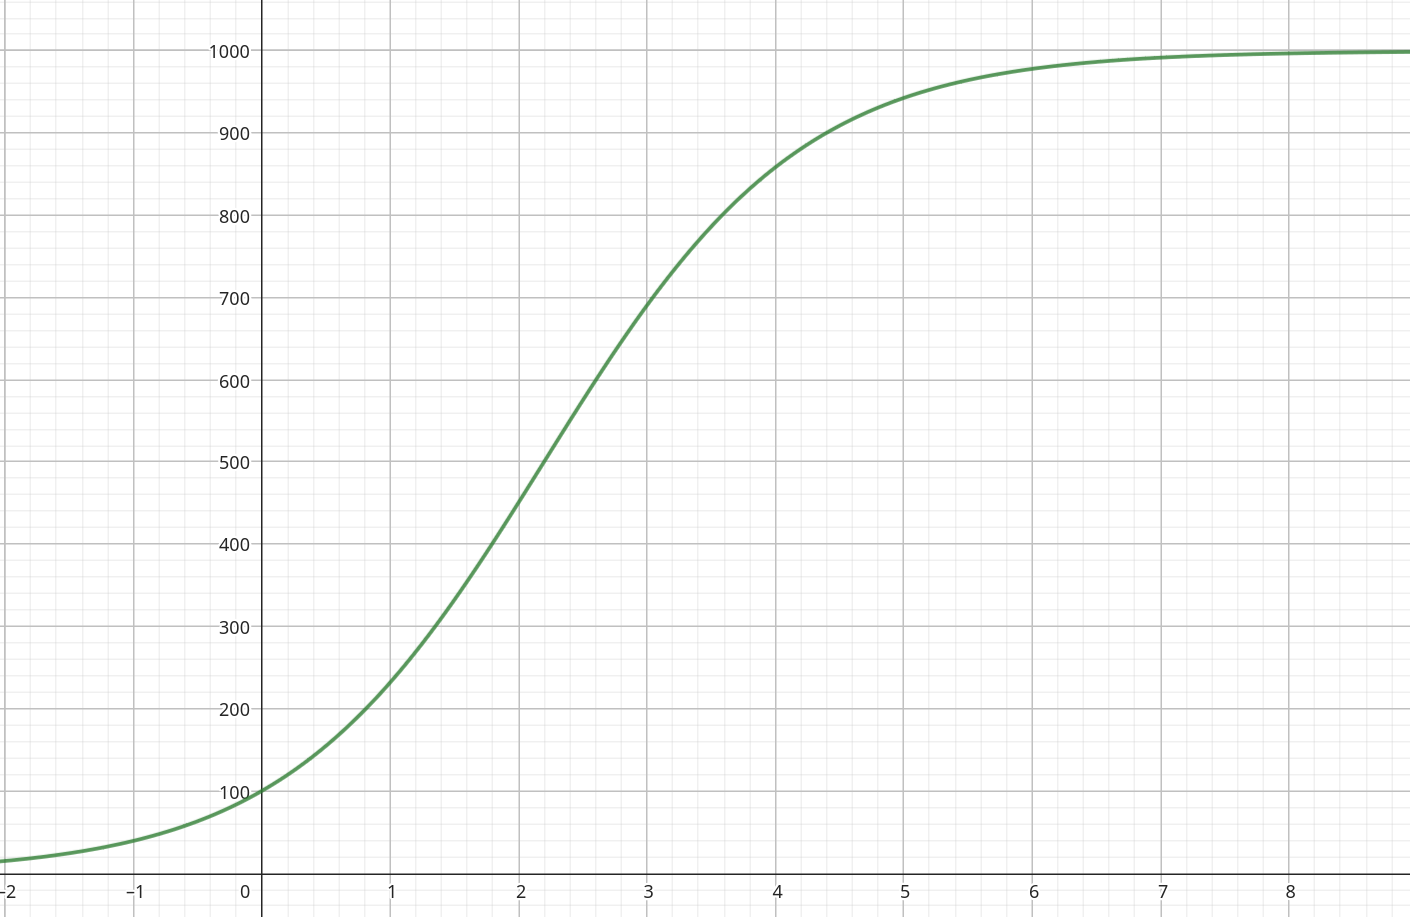
\includegraphics[ width=1\textwidth]{img/graficaPob.png}
\end{figure}
\\
Aprox 4.4 años. $P(4.4) = 900.4984$

\item Encuentre la inversa de esta función y explique su significado.
\[
P = \frac{100 000}{100 + 900 e^{-t}} 
\]
Para encontrar la inversa hay que despejar t
\[
 100 + 900 e^{-t}=\frac{100 000}{P}
\]
\[
e^{-t}=\frac{100 000- 100P}{900P}
\]
\[
t=-ln (\frac{100 000- 100P}{900P} )
\]
\[
\therefore t=-ln (\frac{1 000- P}{9P} )
\]

Entonces, la función inversa es
\[
f^{-1}(t) = t(P) = -ln (\frac{1 000- P}{9P} )
\]
y representa el tiempo requerido t para que la población de ciertas especies alcance un número P.

\item Utilice la función inversa para encontrar el tiempo
necesario para que la población llegue a 900. Compare
con el resultado del inciso \\
\[
f(900) = -ln (\frac{1 000- 900}{9(900)} )=-ln(\frac{100}{8100})=-ln(\frac{1}{81})=-(ln1-ln81)
\]
\[
=ln81+ln1=ln81+0=ln(81) = 4.3944491546724 
\]
$\approx 4.4$ años.
\end{enumerate}


\end{document}